\section{Pestaña de edición de leyes vinculadas}
\label{PEdicionLeyVinculada}

\begin{figure}[H]
\centerline{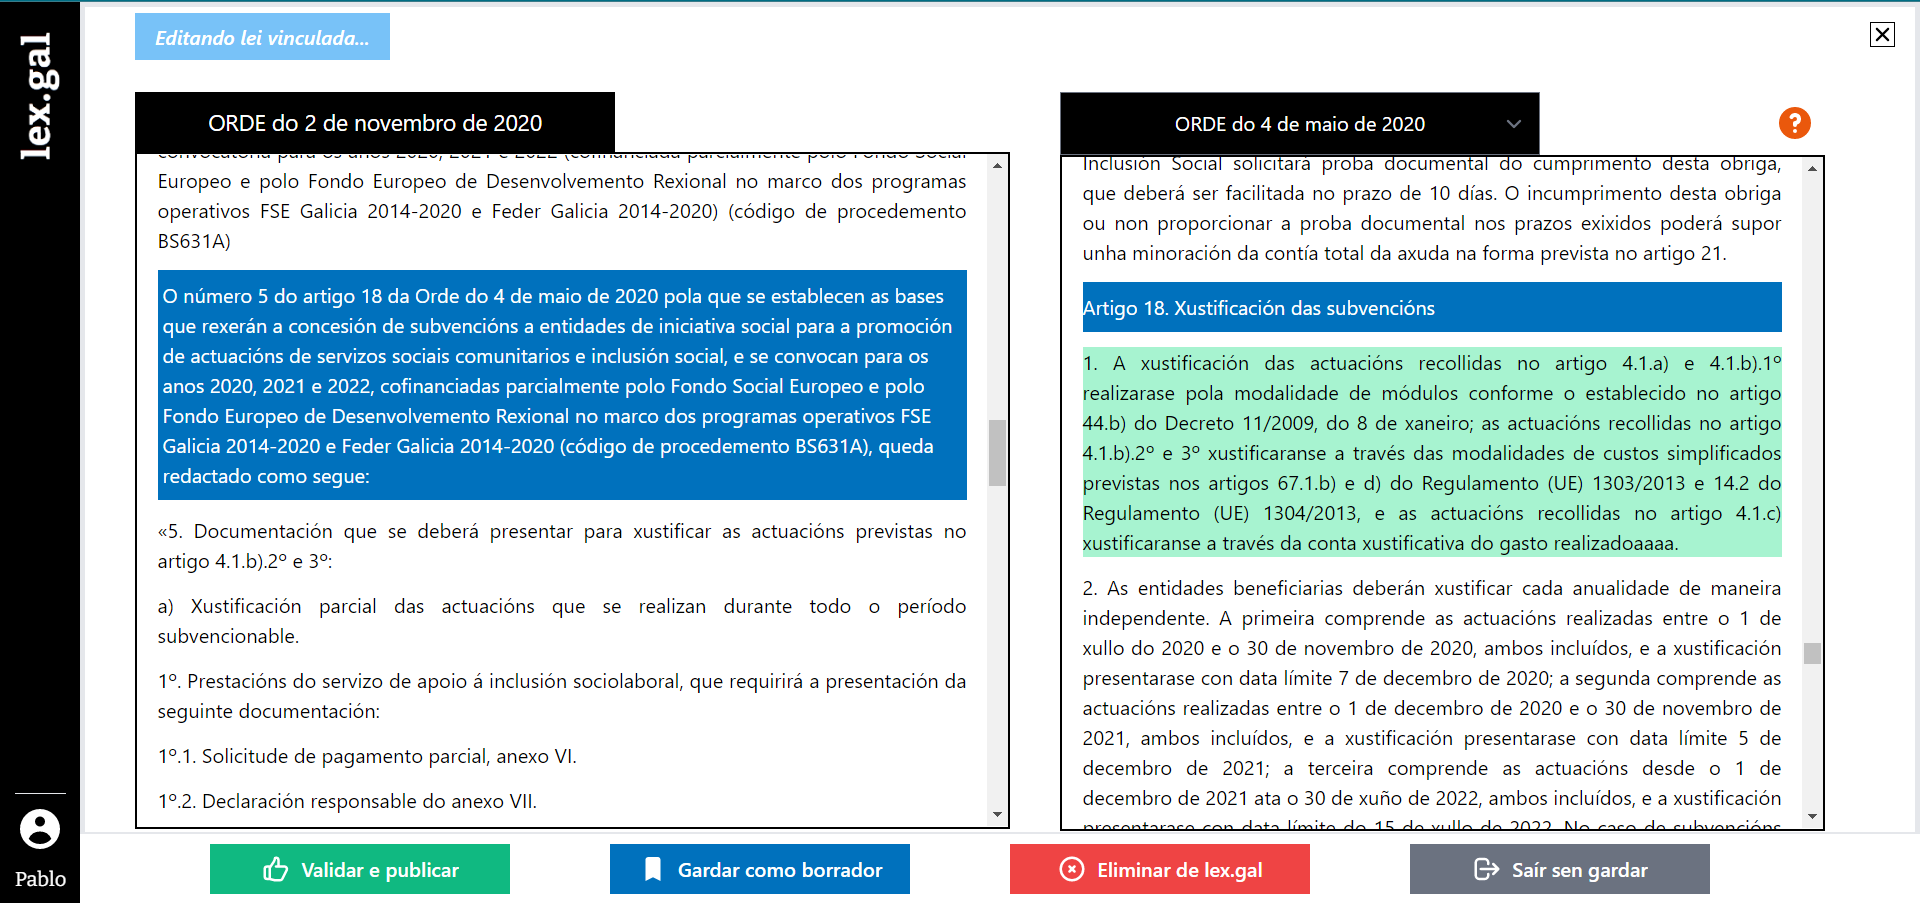
\includegraphics[width=15cm]{figuras/manualUsuario/PestanaLeyVinculada.PNG}}
\caption{Pestaña de edición de leyes vinculadas.}
\label{enlacePLeyVinculada}
\end{figure}

Como última pestaña relacionada con la edición, encontramos la pestaña de edición de las leyes vinculadas. En esta, se muestra la ley principal a la izquierda de la pantalla, y la ley vinculada a modificar a la derecha. En el caso de existir más de una ley a modificar, esta se podría escoger en el seleccionable.
\\

Los párrafos marcados con un fondo de color azul en la ley principal, indican la sección donde se ha de modificar la ley vinculada. Si se pincha sobre este párrafo, se redirige a la parte exacta de la ley vinculada donde se ha de realizar el cambio. Por último, cualquier cambio realizado se marcará con fondo verde. 
\\

Para volver a la pantalla de edición de la ley principal, se ha de cerrar pinchando en la X situada en la parte superior derecha.